Angular momentum of a single particle, $\vec{l}$, is defined as $\vec{r} \times \vec{p}$ where $\vec{r}$ is the position vector and $\vec{p}$ is the momentum vector. Note that $\vec{r}$ depends on the choice of origin, so $\vec{l}$ also depends on the origin.

Similarly torque ($\vec{\Gamma}$) is defined as the rate of change of angular momentum over time. Mathematically, 

\begin{equation*}
    \vec{\Gamma} = \frac{d}{dt}[\vec{l}] = \dot{\vec{l}} = \frac{d}{dt}[\vec{r} \times \vec{p}] = (\dot{\vec{r}} \times \vec{p}) + (\vec{r} \times \dot{\vec{p}})
\end{equation*}

\noindent where $\vec{p} = m \vec{r}$ in the first term, but $\vec{r} \times \vec{r} = 0$ because they are the same line. This makes $\dot{\vec{l}} = \vec{r} \times \dot{\vec{p}}$ but the rate of change of momentum (as defined by Newton's 2nd law) is just the force vector, $\dot{\vec{p}} = \vec{F}$. Compiling this information, we get,

\begin{equation*}
    \vec{\Gamma} = \dot{\vec{l}} = \vec{r} \times \vec{F}.
\end{equation*}

Consequentially, the net torque of a particle also depends on the choice of origin. This is the rotational form of Newton's 2nd law. In one-particle problems, you can choose the origin that the net torque will be equal to zero. In other words, the angular momentum will be constant.

\begin{figure}[h]
    \centering
    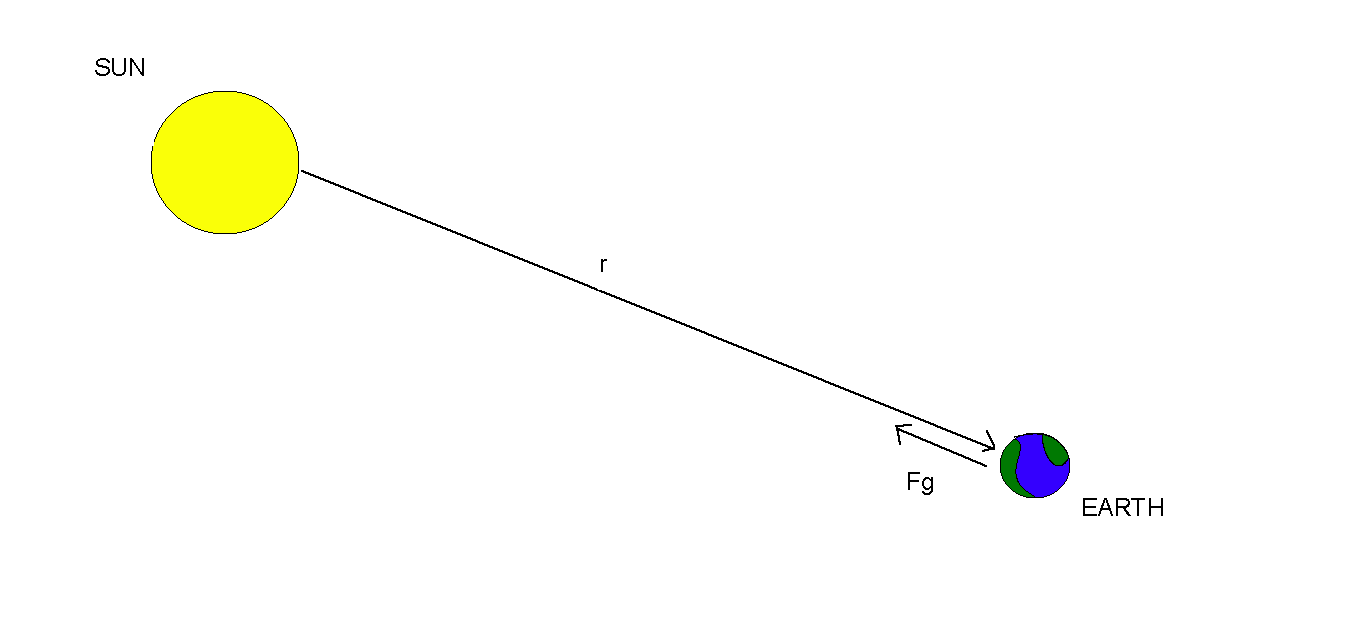
\includegraphics[width=13cm]{Classical_Mechanics/2.6-angular-momentum/torque-earthsun-sys.png}
    \caption{Choosing a smart origin will make analysis much easier.}
    \label{fig:torque-earthsun-sys}
\end{figure}

An example of a smart choice of origin is gravity analysis in planetary systems. Looking at figure \ref{fig:torque-earthsun-sys}, $\vec{\Gamma} = \dot{\vec{l}} = 0, \vec{l} = const.$ This is because $\vec{r} \hspace{1ex} || \hspace{1ex} \vec{F}_g$, thus $\vec{r} \times \vec{F}_g = 0$. Since $\vec{l}$ is constant, $\vec{r}$ and $\vec{p}$ lie in a fixed plane. 3D orbit is reduced to a 2D problem.

Keplers second law of planetary motion is represented in figure \ref{fig:keplers2nd}. It is stated that $PQ$ and $P'Q'$ are separated by equal time and equal area $dt = dt'$ and $dA = dA'$. The area is defined as,

\begin{equation*}
    dA = \frac{1}{2} |\vec{r} \times d\vec{r}| = \frac{1}{2} |\vec{r} \times \vec{v}dt|.
\end{equation*}

Solving for $\frac{dA}{dt}$,

\begin{equation*}
    \frac{dA}{dt} = \frac{1}{2}|\vec{r} \times \vec{p}/m| = \frac{1}{2m}|\vec{r} \times \vec{p}| = \frac{1}{2m}\vec{l}.
\end{equation*}

Since $\vec{\Gamma} = 0$, $\vec{l}$ is constant. With the above result, $\frac{dA}{dt}$ is constant. All central forces have this attribute.

\begin{figure}[h]
    \centering
    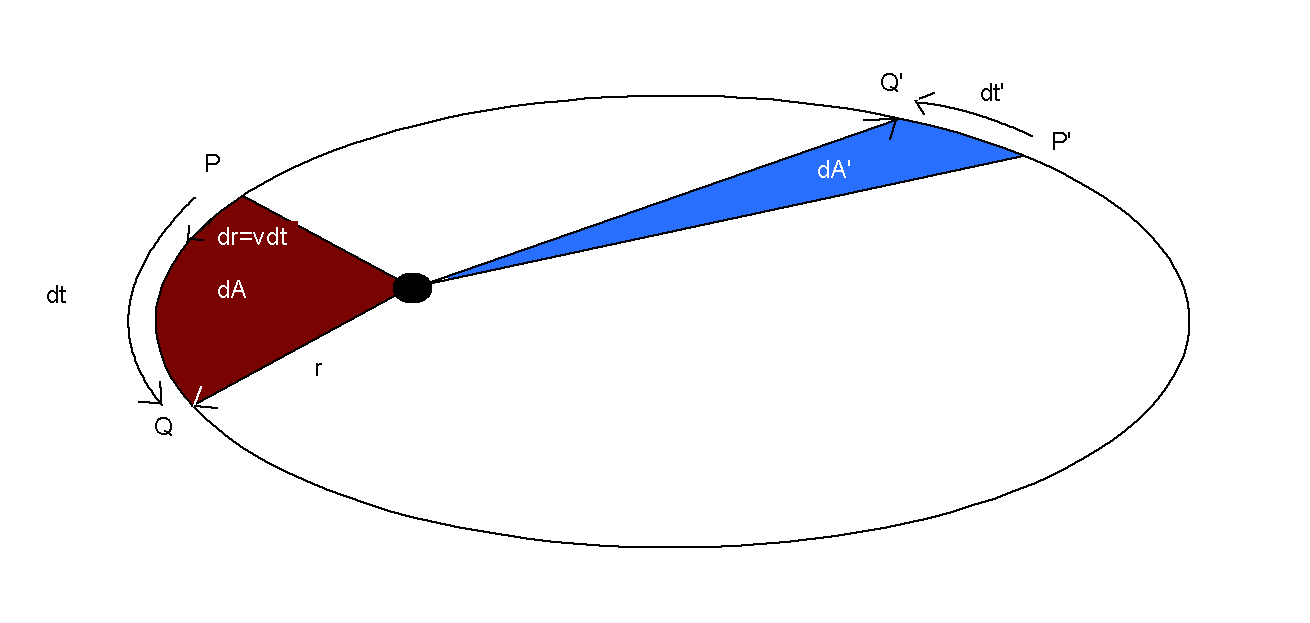
\includegraphics[width=13cm]{Classical_Mechanics/2.6-angular-momentum/keplers2nd.png}
    \caption{If the burgundy area is the same as the blue area, $dA = dA'$, then $dt = dt'$. Keplers second law states that planets sweep out equal area in equal time.}
    \label{fig:keplers2nd}
\end{figure}

It is very simple to expand the current angular momentum definition into any $N$-particle system. A system of $N$-particles, $\alpha = 1, ... , N$, with $\vec{l}_\alpha = \vec{r}_\alpha \times \vec{p}_\alpha$. The total angular momentum of the system is,

\begin{equation*}
    \vec{L} = \sum^N_{\alpha = 1} \vec{l}_\alpha = \sum^N_{\alpha = 1} (\vec{r}_\alpha \times \vec{p}_\alpha).
\end{equation*}

Differentiated with respect to time:

\begin{equation*}
    \dot{\vec{L}} = \sum^N_{\alpha = 1} \dot{\vec{l}}_\alpha = \sum^N_{\alpha = 1} (\vec{r}_\alpha \times \vec{F}_\alpha) = \vec{\Gamma}_\alpha.
\end{equation*}

{\itshape Definition}: {\bfseries Principle of Conservation of Angular Momentum}: Net external, $\Gamma$, on $N$-particle system $=0$, the systems total angular momentum $\vec{L} = \sum \vec{r}_\alpha \times \vec{p}_\alpha = $ constant.

This principle relies on the assumptions that all internal forces (no external forces should exist) are constant and Newtons third law is satisfied (internal forces have equal and opposite reactions to cancel out).

{\exbegin Example 2.6: Putty, Turntable Collision}

The situation is shown in figure \ref{fig:putty-turntable}. The putty is thrown and sticks to the turntable, which rotates the turntable around the z-axis. using the conservation principle, the initial angular momentum $\vec{l}_i = \vec{l}_{putty} = mv = \vec{r} \times \vec{p}$. By definition of the cross product,

\begin{equation*}
    \vec{l}_i = \vec{r} \times \vec{p} = rpsin\theta = r(mv)sin\theta = mvb.
\end{equation*}

The final angular momentum is,

\begin{equation*}
    \vec{l}_f = I\omega,
\end{equation*}

\noindent where $I = I_{putty} + I_{turntable} = mR^2 + \frac{1}{2}MR^2$. Equating the initial and final angular momentums,

\begin{equation*}
    L_{i} = L_f \rightarrow mvb = (m+ \frac{1}{2}M)R^2\omega.
\end{equation*}

Solving for $\omega$ yields $\frac{mvb}{(m+\frac{1}{2}M)R^2}$. This kind of analysis is common in nuclear reactions.

\begin{figure}[h]
    \centering
    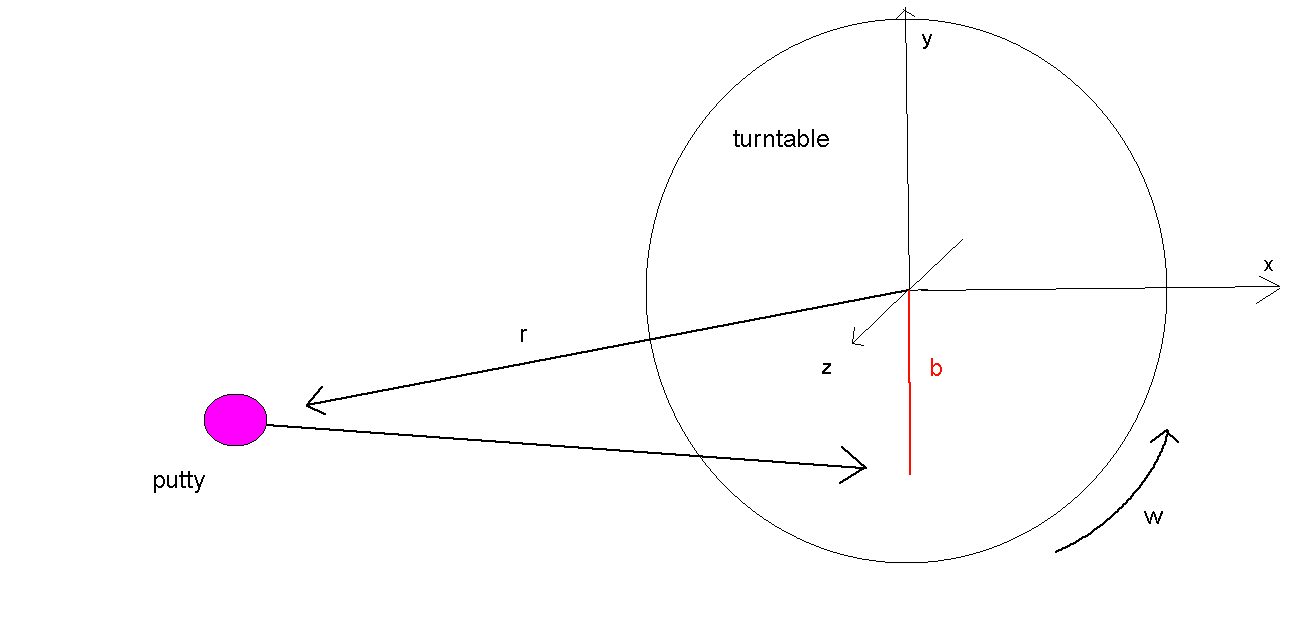
\includegraphics[width=13cm]{Classical_Mechanics/2.6-angular-momentum/ex-putty-turntable.png}
    \caption{Putty-turntable angular momentum example. $\theta$ is not shown, but is the angle of depreciation between the putt and the x-axis.}
    \label{fig:putty-turntable}
\end{figure}

{\exend}